\documentclass[]{resonance}
\usepackage{pgf,tikz}
\usepackage{nameref}
\usepackage{pgfplots}
\usepackage{grffile}
\usepackage{amsmath}
\usepackage{sidecap}
\usepackage{mathtools}
\usepackage{wrapfig}
\usepackage{chemfig}
\usepackage{siunitx}
\usepackage{qrcode}
\usepackage{todonotes}
\usepackage{tabularx} 
\usepackage{amssymb}
\usetikzlibrary{shapes,backgrounds,calc,arrows,arrows.meta}
\pgfplotsset{compat=1.15}

\usepackage[acronym]{glossaries}
%\newglossaryentry{CaM}
%{
%    name=Calmodulin,
%    description={Calmodulin}
%}

\newacronym{camkii}{CaMKII}{calcium/calmodulin dependant protein Kinase II}
\newacronym{cam}{CaM}{calmodulin}
\newacronym{psd}{PSD}{Post Synaptic Densitiy}
\newacronym{ca}{Ca\textsuperscript{++}}{calcium}
\newacronym{pp1}{PP1}{protein phophatase 1}
\newacronym{pp2}{PP2}{protein phophatase 2}
\newacronym{cacam}{Ca\textsuperscript{++}/CaM}{calcium/calmodulin complex}
\newacronym{i1p}{I1P}{phosphorylated inhibitor-1}
\newacronym{i1ppp1}{I1P.PP1}{I1P-PP1 complex}
\newacronym{i1}{I1}{inhibitor-1}
\newacronym{can}{CaN}{calcineurin}
\newacronym{pka}{PKA}{protein kinase A}
\newacronym{darpp}{DARPP-32}{a dopamine- and cyclic-AMP regulated neuronal phosphoprotein}
\newacronym{i2}{I2}{inhibitor 2}
\newacronym{sbgn}{SBGN}{System Biology Graphical Notation}
\newacronym{ltp}{LTP}{Long Term Potentiation}
\newacronym{ltd}{LTD}{Long Term Depression}
\newacronym{nmda}{NMDA}{N-methyl-D-asparate}
\newacronym{nmdar}{NMDAR}{N-methyl-D-asparate receptor}
\newacronym{ampa}{AMPA}{$\alpha$-amino-3-hydroxy-5-methyl-4-isoxazolepropionic acid}
\newacronym{mz}{MZ}{Miller and Zhabotinksy}

\usepackage{xcolor}

\usepackage[]{hyperref}
\hypersetup{
    colorlinks,
    linkcolor={red!50!black},
    citecolor={blue!50!black},
    urlcolor={blue!80!black}
}
\urlstyle{rm}


\newcommand\Fig[1]{\textit{Figure~\ref{#1}}}
\newcommand\TT[1]{\texttt{#1}}

% Title Page
\title{Switches in the brain?} 
\secondTitle{A potential mechanism for long-term memory storage}
\author{Dilawar Singh}
\date{\today}
\begin{document}
\maketitle

% Author info here
\authorIntro{
\includegraphics[width=3.5cm]{./dilawar.jpg}\\
    Dilawar Singh is currently a graduate student at National Center for
    Biological Sciences (NCBS), Bengaluru. His hobby is to convince people to
    move to open-source softwares to live happily ever after.
}

\begin{abstract}
    We forget often. But some memories last a lifetime.
    This means that our brain is capable of protecting memories for years.
    This is a remarkable feat given that the \emph{biochemical hardware}
    involved in creating new memories is a hostile place for
    its storage.  What are the challenges involved? And what type of 
    biochemical mechanisms may overcome them? This article explores a major
    hypothesis that molecular switches may be behind our remarkable ability to
    remember for a lifetime.
\end{abstract}

\maketitle
\monthyear{September 2019}
\artNature{GENERAL ARTICLE}

\section{Introduction}\label{sec:intro}

Our brain is made up of roughly 100 billion neurons, joined together with over
100 trillion connections called \textbf{synapse}s. Each neuron on average makes
1000 connections. It is now widely accepted that persistent changes in these
connections caused by sensory experiences create memories.

\begin{figure}[hb] 
    \centering
    \caption{Memory formation and forgetting. During formation of
        a memory, some synapses become stronger (larger black dots). 
        The longer you can maintain these connections, the longer you 
        can hold on to this memory.
    }\label{fig:engram}
    \framebox{
        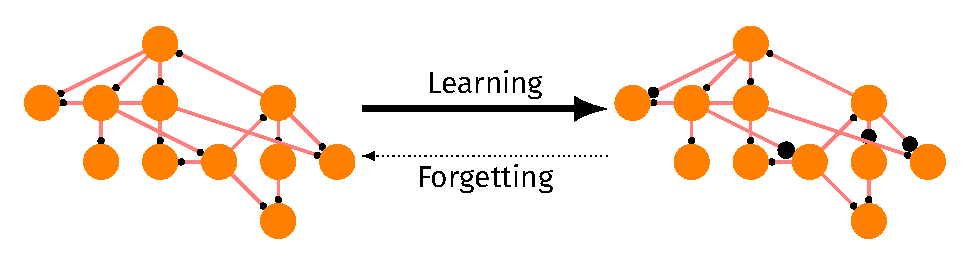
\includegraphics[width=0.95\linewidth]{engram.eps} 
    }
\end{figure}

Let's label these synapses as $s_1, s_2, \ldots s_n$. During memory formation, a
subset of these synapses will undergo changes. For example, my memory of being
chased by a ferocious street dog named \emph{Lalu} (lets call it
$M_\text{Lalu}$) is stored in the set of synapses $M_\text{Lalu}=(s_{10},
s_{21}, s_{12},\ldots,s_{331})$ i.e., these connections were changed during my
troubling encounter with Lalu. I sometimes recall this memory whenever I see a
similar looking dog.

I can recall an experience as long as the set of synapses in which the
particular experience was stored remains intact (\Fig{fig:engram}). Therefore,
our ability to remember is contingent on our brain's ability to keep its
connections intact.  But on the other hand, our ability to learn depends on our
brain's ability to change its connections. And here is the first challenge!

\subsection{Learning quickly v/s forgetting slowly, a zero-sum game}\label{subsec:zero_sum} 
\leftHighlight{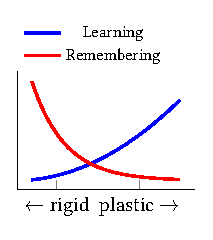
\includegraphics[]{./foget_remember.eps}
Ability to change (plasticity) is good for learning, but bad for remembering.}

For $M_\text{Lalu}$ (or any other memory) to remain intact, each synapse which
participated in its formation (i.e., $s_{10}, s_{21}, s_{12} \ldots$) should
remain intact. The longer a synapse can keep itself unchanged, the better it
will be at keeping the memory safe. Let's assume that somehow I create a synapse
which maintains its state for a very long time (i.e., a rigid synapse). This
synapse will not \emph{forget} easily, but it will not participate in any new
memory formation either. Learning requires synapse to change and a rigid syanpse
can't change.  Rigid synapses behave like a read-only Compact Disk (CD). On the
other hand, if I create a synapse which is easily changeable (i.e., a plastic
synaspe), it will be good at learning new experiences but won't be able to
retain them for long. Plastic synapse forgets easily.  We know that we not only
remember things for long time, we are also capable of learning quickly. And not
just us, most animals are quick to learn. Honey bees can learn the location of a
food source such as flowers after a single encounter. Indeed, a good memory
system is the one which learns as quickly as possible and forgets as slowly as
possible. Forgetting and remembering are two sides of the same coin. They are
conflicting demands i.e., improving one will deteriorate the other -- a zero-sum
game. The challenge is to strike a balance. 

% Hopfield network 
\section{Hopfield network -- associative memory network}\label{sec:hopfield}

Memory storage and retrieval are trivially done by a computer. It will be helpful
to compare memory storage in the computer and the brain. In the computer, we
always know the address of every stored memory, and we access it by providing
this address. The file icon on your desktop is a graphical way of encoding this
addressing scheme. This process is similar to looking up the index page in a
reference book to find a topic. Our brain, on the other hand, is very unlikely
to have such an indexing scheme. 

We recall when we are provided with \textit{cues}. For example, when you see
some part of a familiar person in a wedding album, you could easily identify the
person even though most of the person is hidden behind others.  Many other
memories of that person will also be recalled. A famous class of recurrent
neural network popularly known as Hopfield network can do just the same as shown
in \Fig{fig:hopfield}.
\rightHighlight{Put simply, recurrent networks have \textit{loops}, usually from
output to input.}

\begin{figure}[!b]
    \centering
    \caption{Hopfield network with 100 spiking neurons. These \emph{recurrent} 
        configurations give rise to interesting brain-like
        computation. \textbf{(B)} 6 patterns (memory) i.e. NCBSXY are stored in this
        network. \textbf{(C)} When a very distorted \textit{cue} is applied to
        the network input, it \textit{fetches} one of the stored patterns which is
        the \emph{closest} to the applied cue.
    }\label{fig:hopfield}
    \framebox{
        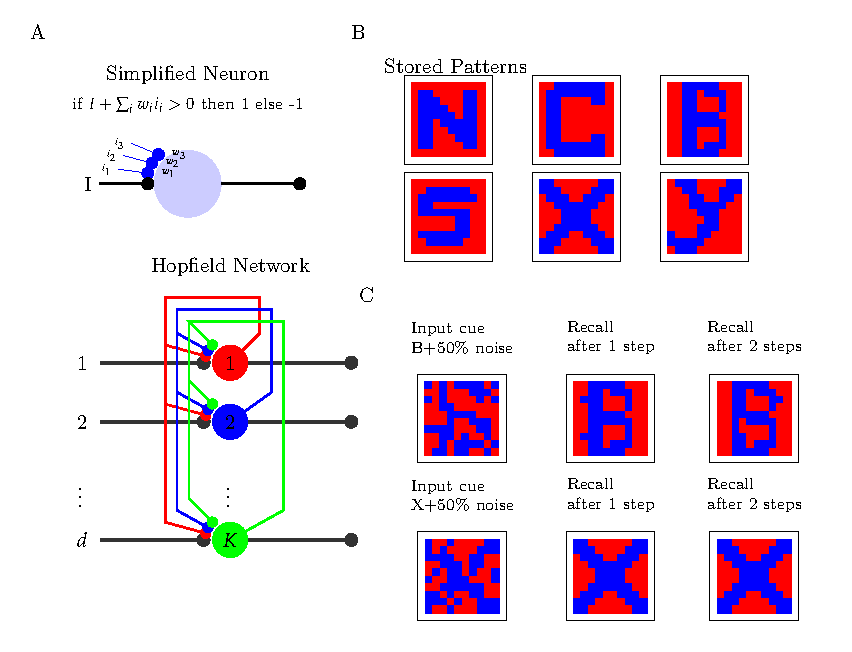
\includegraphics[width=0.95\linewidth]{./hopfield.eps}
    }
\end{figure}

How this recurrent network works is beyond the scope of article. Readers are
encouraged to explore more by themselves. \emph{``How well can we explain
biological memory using these networks?''} is an active research area.  Though
these networks are extremely successful in accomplishing various
\textit{brain-like} computations (\textit{a la} machine learning), I would like
to advise the reader to be skeptical by noting the following:

\begin{itemize}
    \item  Neurons used in these networks are highly simplified. \textit{Real}
        neurons are not this simple. Even though these simplified neurons
        capture the essential \textit{all-or-none} (electrical spike) way of
        communication and learning by changing synaptic connections, they do
        ignore rich local computations which can be accomplished by branches of
        these neurons called \textit{dendrites}.
    \item  There is no evidence that neurons make such dense recurrent
        connections. However, some studies have shown that Hopfield network can
        work with very sparse recurrent connections as well.
    \item Activity in these networks does not match the usually observed activity 
        in the primate brain during memory-recall experiments.
\end{itemize}

\leftHighlight{Solutions proposed by other disciplines often provide very useful
    insight, but in the end, all solutions must work well under the constraints 
    imposed by biology and chemistry.
}

Nonetheless, these networks provide us with a framework to concretely think
about the problem of memory storage and recall. We learn a great deal about a
problem by pointing out the limitations and failures of models which describe it. 

Hopfield network has properties which will sound very natural to us. Can you
store as many memories as you like in these networks? No. There is an upper
limit. Adding more patterns over the maximum limit distorts memories.  When a
cue is given, the network no longer fetches the right pattern. It often fetches
a pattern which was not even stored; the retrieved pattern instead resembles
some mixture of stored patterns. When too many memories are stored, they corrupt
each other by mixing up. One can ask more questions. When connections decay in
these networks and memories start disappearing, which memory disappears first:
the weakest or the newest? And, when a new memory closely associated with an old
memory is added, what happens to those old memories?

After this necessary detour, let us go back to the main theme: how do synapses
maintain their state?

\section{How does a synapse maintain its state?}

Very complex biochemistry plays out during learning that changes the synapse.
Surprisingly, the net effect of this complex biochemistry can be summarised by a
simple mathematical expression. Ah, \emph{the unreasonable effectiveness of
mathematics} \cite{unreasonable_math}! Let's assume that synaptic strength $w$ is
tightly correlated with a chemical species $X$ found at the synapse i.e. $w$ changes
with $X$. Therefore, the problem of ``\emph{synapse
maintaining its state}'' becomes the problem of ``\emph{molecule $X$ maintaining
its state}'' -- a more concretely defined problem.

Let's assume that $X$ is converted to its active form $X^*$  by adding a
\rightHighlight{ \raggedright 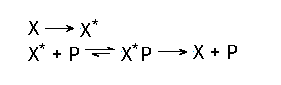
\includegraphics[width=3.5cm]{./fig_model.eps} }
phosphoryl group ($PO_3^{2-}$). The phosphoryl group is removed by a phosphatase
and $X^*$ is turned back into inactive $X$. Phosphorylation and its
counterpart dephosphorylation are very common motifs for controlling various
chemical reactions by activating and deactivating protein molecules. Once most
$X$ has been turned into $X^*$ during memory formation, how do we make sure that
$X^*$ does not turn back into $X$ (lose memory)?

Let's mull over a solution to this problem of long term maintenance of $X^*$.
Here is one potential solution. Can you think of any other solution?

\begin{enumerate}
    \item \textbf{Amplification:} $X^*$ \textbf{auto-phosphorylates} itself i.e. \tikz[baseline]{ 
            \node (x) {$X$};
            \node[right=9mm of x] (xp) {$X^*$};
            \draw[-latex] (x) -- (xp);
            \draw[-latex] (xp) edge[out=120, in=90] ([xshift=7mm]x);
        }. If we manage to get sufficient $X^*$ somehow, it
        will act as a catalyst to its own production. $X^*$ will always remain
        high.
    \item Dephosphorylation of $X^*$ is minimized by controlling the number of
        phosphatase ($P$) or by reducing the reaction rate.
\end{enumerate} 

Both (1) and (2) help in making $X^*$ highly stable. Problem solved? No.  Now
we have constructed a rigid synapse. Recall the \textit{rigid} v/s
\textit{plastic} synapse dilemma discussed previously (section
\ref{subsec:zero_sum}). This synapse will definitely remember for longer
but it will not participate in any new learning anymore.

As long as we are in the realm of theory, let's propose a solution to this
problem. We add another reaction say $P'+X^*\rightarrow P'X \rightarrow P'+X$
which deactivates $X^*$ when the \textit{need} arises. Phosphatase $P'$ is
different from $P$. This adds another layer of control to an already complicated
problem i.e., forgetting is now controlled by another process. This requires one
more explanation: how does this new mechanism controlling \textit{forgetting}
work?  And philosophically -- if you care about it -- it violates the principle
of \textbf{parsimony} which recommends picking the simplest explanation.

We still have two big problems hiding underneath. We have not considered the
underlying biological hardware i.e. synapse in any detail where this biochemical
network is supposed to function. The first problem is \emph{chemical noise}. For
a biochemical system operating in very small volume, effect of chemical noise
can be very strong. \leftHighlight{The volume of a typical synapse is
$\sim$\SI{e-20}{\cubic\meter}. At this volume, \SI{1}{\micro M} concentration is
roughly equal to 6 molecules!} There are over 200 types of protein molecules in
a typical synapse. Indeed, most proteins found at synapse has copy number as low
as few tens. The brain is always active and the chemical noise caused by the
brain's background activity will surely turn some molecules of $X$ into $X^*$.
Then due to auto-phosphorylation, sooner than later, all $X$ will be turned into
$X^*$. As a result, we have created a very stable memory of nothing but
background noise.  This is highly undesirable!

The second problem is \textit{turnover} i.e., old molecules are continuously
degraded and being replaced by newly minted molecules. Let's assume that at the
time of memory formation, we had 100 molecules of $X^*$ in the synapse and, on
average, every day one newly formed molecule replaces an
old one ($X^* \rightarrow X$).  After 50 days, half of the synaptic strength is
gone! To counter this, we must have a \textit{refresh} mechanism by which the
newly added molecule quickly changes its state according to the state of synapse
i.e., newborn $X$ becomes $X^*$ if most molecules at the synapse are $X^*$.

\begin{figure}[]
    \centering
    \caption{A hypothetical network which can solve the problem of chemical noise and
        turnover with suitable parameters. The activation step is divided
        into slow and fast components such that fluctuations caused by background
        noise do not cause the system to activate itself. $X^*$ also partially
        activates $X$ to $X^\sim$ to overcome \textit{turnover.}
    }\label{fig:model_bistable}
    \framebox{
        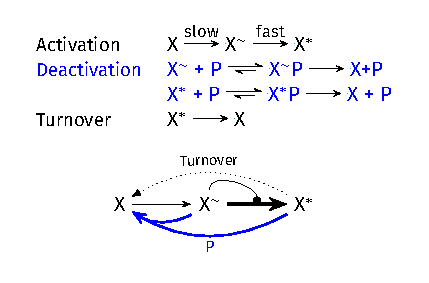
\includegraphics[width=0.95\linewidth]{./fig_model_b.eps}
    }
    \vspace{2mm}
\end{figure}

Effectively, we want a stable \texttt{ON} state (all $X$ are $X^*$) which is
immune to turnover. We also want a stable \texttt{OFF} state so that noise does
not turn $X$ into $X^*$.  We want a switch-like behaviour i.e., if it is
\texttt{OFF} or \texttt{ON}, it tends to stay \texttt{OFF} or \texttt{ON}. If a
few $X$ are turned into $X^*$ by background noise, we want them to be quickly
turned back into $X$ by the phosphatase $P$. And if during memory formation, a
significant portion of $X$ has been turned into $X^*$, then we want that any
$X^*$ deactivated into $X$ is quickly activated again into $X^*$. This system
should operate like a switch which does not flip unless significant force is
applied. This is called \textbf{bistable switch}.

Is there any evidence that bistable chemical reaction networks exist? Do they
occur at all in living cells?  What is the reason for their \emph{selection} by
evolution? And what do they accomplish? (see \textit{Box 1})
\rightHighlight{Bistability (and its close relative -- oscillations)
is very common in biology from cellular level (genetic switch) to population
levels (predator-prey dynamics).}  

Bistability, from one point of view, is an irreversible way of taking YES or NO
decisions. A phage $\lambda$ virus can use it to decide if to remain dormant or
become active; a cell can use it to decide whether to move to M phase from G1
phase or whether to enter apoptosis or not. From another point of view,
bistability is a way to store 1 bit of memory (1 and 0, \texttt{ON} or
\texttt{OFF}, \texttt{ACTIVE} or \texttt{INACTIVE}). \emph{Memory is older than
brain!} There are plenty of living organisms without brain as we define them but
I can't imagine a living organism without memory. So it won't be surprising if
we discover bistable switches operating at synapses as well. Indeed, various
studies have shown that \gls{camkii} (see \textit{Box 2}) \emph{may} form
bistable switches in the synapses. 

% box here.
% Bistable box
\boxTexteven{Bistability in reaction network}
{
    \def\StateA{\tikz \node[circle, dashed, draw, inner sep=1pt] {\scriptsize
    \textsf{A}};}
    \def\StateB{\tikz \node[circle, dashed, draw, inner sep=1pt] {\scriptsize
    \textsf{B}};}

    In a world full of fluctuations, stability is indeed a very useful property.
    Life is remarkably stable even though it is made up of inherently noisy
    components. Bistable chemical networks are ubiquitous in biology. In
    bistable chemical networks, noisy components acts together to give rise to 
    highly (bi)stable behaviour. \emph{Also note that even though the underlying
    reactions are almost always reversible, the bistable switch is usually not
    reversible}. Isn't it a neat way to make a very decisive cell?

    A bistable system -- as its name implies -- has two stable states. From the
    point of view of an experimentalist, if you obverse a bistable system for
    a very long time, you would almost always find it in either of its two stable
    states. Just like an electrical switch which you would almost always find in
    either \texttt{ON} or \texttt{OFF} state (and rarely in transition between
    states).

    \vspace{2mm} 
    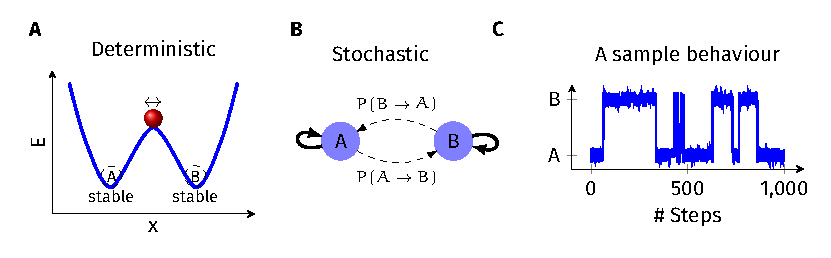
\includegraphics[width=\linewidth]{./stability_noise.eps} 
    {\footnotesize \textbf{(Figure A)} 
        \textbf{(i)} A conceptual model of bistability.  The
        energy landscape of a bistable system has two minima (\protect\StateA and
        \protect\StateB), therefore, the system always ends up in either of them. It is a
        deterministic bistable system. \textbf{(ii)} A conceptual representation
        of stochastic bistable system as state transition diagram.  The arrows
        depict the probability of transition from one state to the other. In
        \textbf{(iii)} We simulate the system described in \textbf{B} with probability
        of transition from A to B ($P(A\protect\rightarrow B)$), and from B to A
        ($P(B\protect\rightarrow A)$) set equal to 0.01.
    }

    \vspace{2mm}
    Such bistable motif are commonplace in biology \cite{ramakrishnan2008},
    especially found in situations where cell has to make a decision or store
    information (memory). One such motif is shown below in both deterministic
    and stochastic settings. 

    \vspace{2mm}
    \begin{center}
    \begin{tikzpicture}[scale=1 , every node/.style={} ]
        \node[] (img) {
                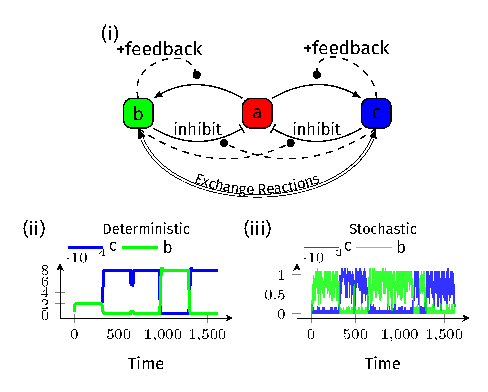
\includegraphics[width=6cm]{./strong_bis_naren_and_bhalla_87mm.eps}
            };

        \node[right=5mm of img.south east, anchor=south west, text width=6cm, align=justify] 
            {
                \footnotesize
                \textbf{(Figure B)}
                \textbf{(i)} A bistable chemical system adapted from \cite{ramakrishnan2008}.
                Species \texttt{b} and \texttt{c} catalyze their production
                (positive feedback) and inhibits production of \texttt{a}.
                Two trajectories are shown in different
                settings. \textbf{(ii)} System is deterministic; \textbf{(iii)} System is stochastic.
                There are three necessary conditions a network must have to be able to show
                bistability: positive feedback, mechanism to filter out small stimuli, and a
                mechanism to prevent explosion \cite{wilhelm}. 
            };
    \end{tikzpicture}	
\end{center}
}


\section{Molecular bistable switch at synapse}\label{sec:molecular_switch}

Late John Lisman hypothesised that a kinase and a phosphatase together can form
a bistable switch immune to \emph{turnover}. \gls{camkii} and its phosphatase
\gls{pp1} were identified as the hypothesised kinase and phosphatase. This
chemical system has been extensively studied using computational models for over
two decades \cite{sandstorm}. There is some evidence that \gls{camkii} is
bistable \emph{in vitro} conditions. Whether \gls{camkii} is bistable inside a
living neuron is still an open question (see \textit{Box 2} for an overview of
\gls{camkii} properties at a synapse.).

\rightHighlight{
    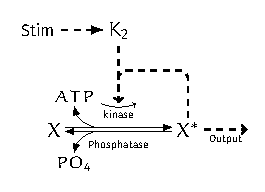
\includegraphics[width=4cm]{./lisman_bistable_small.eps}
    Reaction in a bistable switch proposed by John Lisman. Modified
    from \cite{lisman1985}.
    \label{fig:lisman}
}

In our computational study of this pathway, we explored the effect of subunit
exchange on \gls{camkii} pathway \cite{SinghAndBhalla2018} (see \textit{Box 2}).
A \gls{camkii} molecule is made up to 12 to 14 subunits which it can exchange
with other molecules. This makes \gls{camkii} a rare molecule, perhaps unique.
Subunit exchange enables \gls{camkii} to act at a position away from its current
location. Due to its unique properties, \gls{camkii} is often called \emph{the
memory molecule}.

\gls{camkii} acts as an integrator of calcium activity. The capacitor is a good
example of an integrator. The potential across its terminal $V$ is given by
$\frac{1}{C}\int i\; dt$ i.e., a capacitor integrates current. By measuring
voltage across the ideal capacitor at time $t$, you can tell how much current
must have passed through it till time $t$. That is, you can tell the
\emph{history} of current by measuring the present value of voltage. Integrators
can also be used to store information. 
\rightHighlight{
    A leaky integrator \emph{leaks} the stored variable 
    , just like a leaky bucket which leaks water or a leaky capacitor which
    leaks charge. After some time, any stored variable will be lost forever.
} 
Indeed, in many storage devices, a fully
charged capacitor represents bit 1 and a discharged capacitor represents bit 0.
The real world capacitors are \emph{leaky} -- they leak charge and information
is lost after some time. So devices which use them to store information has to
periodically recharge these capacitors.

\begin{figure}[]
    \centering
    \caption{ \textbf{(A)} (left) Three clusters of \gls{camkii} in a synapse
        . (right) This system's ability to hold memories increases exponentially
        with the system size: 52 holoenzymes can keep the memory intact roughly for
        100 years! \textbf{(B)} Subunit exchange improves \gls{camkii} ability
        to store information. \textbf{(Red)} 3 individual bistable switches independently  
        without subunit exchange. \textbf{(Blue}) When subunit exchange is enabled, these 
        independent switches synchronize. Notice that the now the system spends more 
        time in its stable states.
    }\label{fig:camkii_sync}
    \framebox{
        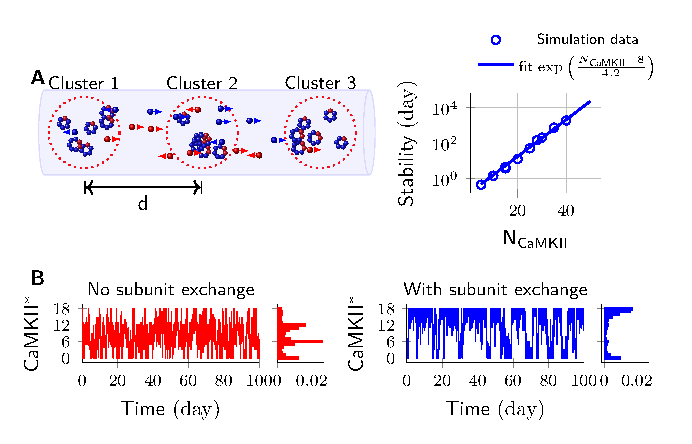
\includegraphics[width=0.95\linewidth]{figure_sync_114mm.eps}
    }
    \vspace{3mm}
\end{figure}

Like a capacitor, \gls{camkii} also integrates. It integrates \gls{ca} activity
i.e., $[CaMKII]=\int [Ca]\; dt$.  By measuring \gls{camkii} activity, one can
estimate the history of \gls{ca} activity. But just like a real world capacitor
which leaks charge, \gls{camkii} also leaks. A single \gls{camkii} ability to
retain information is bounded by this leak -- it roughly last a minute.

We found that the subunit exchange improves information retention capacity of
\gls{camkii}. Individual \gls{camkii} acts as leaky integrator of \gls{ca}
activity (see \textit{Box 2}). With subunit exchange, the leaky integrator
becomes less leaky because of cooperation among holoenzymes. An active
holoenzyme can help its neighbour remain active for a longer period by
exchanging active subunits with it. As a result, a \gls{camkii} close to an
active \gls{camkii} can retain its active state for a longer time.

Moreover, \gls{camkii} holoenzymes often come together and forms a cluster. The
behaviour of a cluster could be very different than the behaviour of individuals
in it (\emph{emergent property}). \leftHighlight{The behaviour of a
school of fish could be very different from any fish in it.\linebreak
\qrcode[height=2cm]{https://youtu.be/Y-5ffl5_7AI} } The clustering of
\gls{camkii} give rise to a bistable switch (\Fig{fig:camkii_sync}). Such
clustering by various molecules have been observed in experiments and is now
thought to play a very important role. We found that subunit exchange
synchronizes bistable activity of distributed clusters. That is, multiple
bistable switches act as a single but much more stable bistable switch. In
nutshell, we found the subunit exchange makes \gls{camkii} molecule better at
retaining information.


% CaMKII box.
\boxTextodd{\gls{camkii} at synapse: A brief overview} {

    \gls{camkii} constitutes roughly 2\% of more than 2000 proteins found in
    brain. It is enriched in the hippocampus -- a brain structure necessary for
    memory formation. Indeed, \gls{camkii} is known to play an essential role in
    learning and memory. In experiments involving mice, deactivating
    \gls{camkii} in any way has always resulted in the impairment of memory
    formation and learning. 

    \gls{camkii} molecule has interesting properties which makes it an
    attractive candidate for storing information. It is unique among proteins
    for its dodecameric/tetradecameric structure (A, structure from Protein Data Bank),
    its ability to exchange part of it with others (B) and its complex response
    to calcium signal.  Usually it acts as a integrator of calcium activity in
    synapse (C).

    \vspace{2mm}
    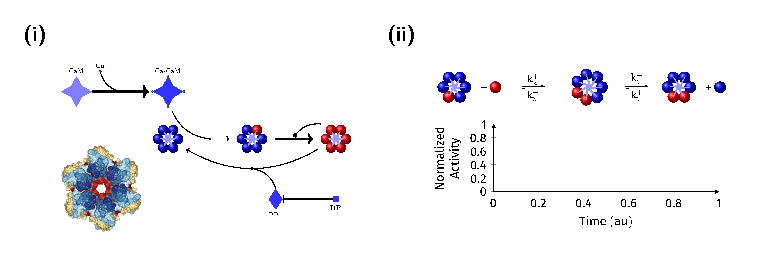
\includegraphics[width=0.9\linewidth]{./camkii_properties.eps} \\
    \textbf{Figure C.} \textbf{(i)} Summary of \gls{camkii} pathway. Upon its influx into
    the synapse, \gls{ca} binds to \gls{cam} and creates a complex \gls{cacam}.
    \gls{cacam} binds to \gls{camkii} and phosphorylate it's subunit (red
    balls). \gls{camkii} is dephosphorylated by \gls{pp1}. \textbf{(ii)} Subunit
    exchange between two holoenzymes i.e., a fully active \gls{camkii} holoenzyme
    can lose an \textit{ACTIVE} subunit which can be picked up by another
    holoenzyme which becomes partially active. 
    
    \vspace{2mm}
    Activation of \gls{camkii} requires two steps: the first step is very slow
    for it requires binding of two \gls{cacam} simultaneously. Once a subunit
    has been activated (red ball), phosphorylation of its neighbours requires
    binding of only one \gls{cacam} and, therefore, second step proceeds at  much
    faster rate.  Note that the first very slow step can be overcome by subunit
    exchange when an inactive holoenzyme picks up an active subunit released by
    other holoenzyme. Thus subunit exchange helps in spreading \gls{camkii}
    activation. 

    \textbf{\gls{camkii} integrates \gls{ca} signal:} A single \gls{camkii}
    holoenzyme acts as a leaky integrator of \gls{ca} activity i.e., it sums up
    \gls{ca} activity in time. And it also decays with a time-constant (leaky).
    See \textbf{(ii)} to compare the behaviour of three integrators of calcium
    activity ($x$): a non-leaky integrator and two leaky integrators with small
    and large amount of leakage. Mathematically, it is similar to a leaky
    capacitor charged by current source. Integrators are useful when you want to
    accumulate \emph{enough} information about something (say $x$) before taking
    a decision e.g.  a plant can \emph{decide} to flower or shed leaves only if
    integration of moisture in air and/or temperature during the day crosses a
    threshold value.

} % box

\begin{figure}[h!]
    \centering
    \caption{\textit{All-or-none} v/s graded synapse and mechanism which may
        give rise to them. \textbf{(A)} A bistable mechanism (red) controlling the 
        synaptic strength (blue). Synaptic strength changes in \textit{all-or-none}
        fashion. \textbf{(B)} A multi-stable mechanism (red) gives rise to a
        graded synapse (blue). Synaptic strength changes in a step-wise manner. Note that 
        a multi-stable mechanism can be constructed by adding multiple bistable
        switches. In this case, 4 bistable switches were used (shown in light
        blue in background. Red curve is the algebraic sum.).
    }
    \framebox{
        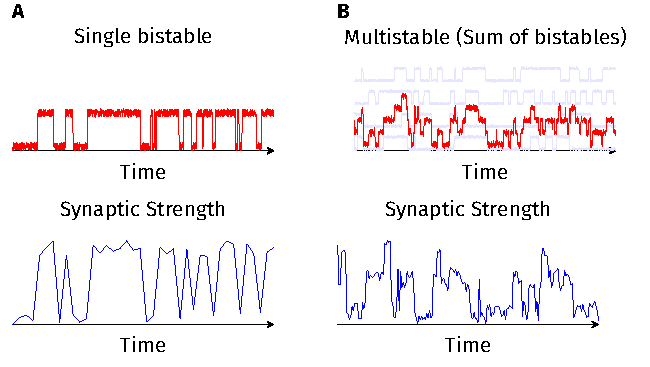
\includegraphics[width=0.9\linewidth]{./bistable_multistabe_synapse.eps}
    }
    \label{fig:fig_bistable_multistable}
    \vspace{2mm}
\end{figure}


% References section
\section{Conclusion} 

In this article, we have discussed why bistable motif is an attractive candidate
for storing biological memories (\textit{Box 1}). They are ubiquitous in biology
and are natural solution to the problem of memory maintenance under chemical
noise and turnover.  We have also discussed a potential pathway (\gls{camkii})
which may be bistable at synapses. Now let's put all of this to a reality check.
Let's assume that bistables mechanism exists at synapses. If the underlying
mechanism is bistable, then I \emph{must} observe a bimodal distribution. We
know that the size of a synapse is tightly correlated with its strength. That
means we can observe synapse size as the proxy of its strength.  If we observe
synapse for a long time and record its size continuously, what would we observe
if our hypothesis is correct? If size distribution is bimodal (two peaks) then
it is a strong suggestion (not a proof!) that underlying mechanism is bistable. 

There is now growing experimental evidence that synaptic size change in
\textit{all-or-none} (\texttt{ON} and \texttt{OFF}O) manner, a finding which is
consistent with the idea of synaptic switch. Some other studies have claimed
that changes are graded i.e., synapse changes in a step-wise manner much like a
\textbf{multi-stable} synapse. A multi-stable synapse is an additive ensemble of
many bistable components (\Fig{fig:fig_bistable_multistable}).


Whether \gls{camkii} is bistable in the synapse is still an open question;
neither there is any concrete evidence that it is nor it has been ruled out that
it is not, especially near the membrane. Our aim in this article was to point
out why the bistable mechanism is a viable solution to the problem of storing memory
for long time. Even if \gls{camkii} turns out not to be bistable at synapse,
there could still be other mechanisms which are bistables -- a few of them have
been proposed. Given that bistable chemical motifs are widespread, it is
reasonable to suggest that there are indeed switches in our brain -- much like
flip-flops in the digital memory card of your phone -- which are evolved to keep
our memories safe from the onslaught of time and noise.

\rightHighlight{
    \begin{tabular}{p{4cm}}
    \qrcode[height=2cm,hyperlink]{https://gitlab.com/dilawar/Resonance2018}  \\ \\ 
    Simulations presented in this article are available here.
\end{tabular}
}

\section*{Acknowledgements} I'd like to thank Dr. Somya Mani, Bhanu Priya and
Dr. Mukund Thattai for helpful suggestions on the manuscript. 

\vspace{3mm}
\correspond{
    Bhalla Lab,
    National Center for Biological Sciences, Bengaluru \\
    GKVK Campus, Bellary Road \\
    Bengaluru - 560065.  \\
    Email: dilawars@ncbs.res.in
}

\begin{thebibliography}{99} 

    \bibitem{unreasonable_math}
    Eugene Wigner,
    \textit{The Unreasonable Effectiveness of Mathematics in the Natural Sciences},
     Communications in Pure and Applied Mathematics, vol. 13, No. I (February 1960)

    \bibitem{ramakrishnan2008}
    Naren Ramakrishnan, Upinder S. Bhalla
    \textit{Memory Switches in Chemical Reaction Space},
    PLOS Computational Biology, No 7 vol. 4 (July 2008)

    \bibitem{wilhelm}
    Thoman Wilhelm,
    \textit{The smallest chemical reaction system with bistability},
    BMC Systems Biology, vol. 3, No 1 (Sep 2009)

    \bibitem{sandstorm} 
    Malin Sandstorm,
    \textit{Models of CaMKII activation},
    Master Thesis, Royal Institute Of Technology Sweden 

    \bibitem{SinghAndBhalla2018}
    Dilawar Singh, Upinder S Bhalla,
    \textit{Subunit exchange enhances information retention by CaMKII in dendritic spines},
    eLife, doi:10.7554/eLife.41412

    \bibitem{koch1999}
    Christof Koch
    \textit{Biophysics of computations}.
    Oxford University Press, 1999

    \bibitem{lisman1985} 
    Lisman J. E., 
    \textit{A mechanism for memory storage insensitive to molecular turnover: a
    bistable autophosphorylating kinase}. 
    Proc. Natl. Acad. Sci. USA, May 1985


    \bibitem{stratton}
    Stratton M et al.,
    \textit{Activation-triggered subunit exchange between CaMKII holoenzymes
    facilitates the spread of kinase activity}, Elife (Jan 2014) 

\end{thebibliography}

\end{document}
